%\documentclass{emulateapj}
\documentclass[letterpaper,12pt,preprint]{aastex}

% packages
\usepackage{amssymb,amsmath,amsbsy}
\usepackage{bbold}
\usepackage{arydshln}
\usepackage{algpseudocode}
\renewcommand\algorithmicthen{}
\renewcommand\algorithmicdo{}

% commands
\newcommand{\given}{\,|\,}
\newcommand{\dd}{\mathrm{d}}
\newcommand{\transpose}[1]{{#1}^{\mathsf{T}}}
\newcommand{\inverse}[1]{{#1}^{-1}}
\newcommand{\msun}{\mathrm{M}_\odot}
\newcommand{\bs}[1]{\boldsymbol{#1}}
\newcommand{\ident}{\mathbb{1}}

\newcommand{\act}{J}
%\newcommand{\jac}{\bs{\rm J}}
\newcommand{\jac}{\bs{G}}

\begin{document}

\title{Tidal streams in triaxial systems}
\author{Adrian M. Price-Whelan\altaffilmark{\colum,\adrn},
	    Kathryn V. Johnston\altaffilmark{\colum},
	    Monica Valluri\altaffilmark{\mich}}

% Affiliations
\newcommand{\colum}{1}
\newcommand{\adrn}{2}
\newcommand{\mich}{3}
\altaffiltext{\colum}{Department of Astronomy, 
		              Columbia University, 
		              550 W 120th St., 
		              New York, NY 10027, USA}
\altaffiltext{\adrn}{To whom correspondence should be addressed: adrn@astro.columbia.edu}
\altaffiltext{\mich}{ }

\begin{abstract}

Tidal streams form from the steady disruption of stellar systems
orbiting within the gravitational field of some parent galaxy. Many
streams and debris structures have been discovered in the halo of the
Milky Way and have been used to model the potential of the Galaxy. 
However, few of these models have yet explored the properties of
tidal debris in triaxial potentials.
The existence of a variety of orbits, resonances, and chaotic regions in such potentials 
suggest that the morphologies and dispersal timescales of
debris could differ significantly from the simpler spherical and oblate cases.
In this work we use a series of N-body simulations of stellar systems over a range 
of masses of disruption in triaxial potentials to understand the influence of the nature 
and types of orbits on debris morphologies.
Our results suggest that the mere existence of the multitude of thin streams
already known to orbit the Milky Way provides significant constraints on the
classes of triaxial potentials that provide a good representation for its dark matter halo.

\end{abstract}

\keywords{
}

%\begin{figure*}[!h]
%\begin{center}
%\includegraphics[width=\textwidth]{PATH}
%\caption{ CAPTION }\label{fig:FIGNAME}
%\end{center}
%\end{figure*}

\section{Introduction}\label{sec:introduction}

Adding third degree of freedom opens up many new orbits / resonances / etc. -- Valluri and Merritt work...

The halos of galaxies are filled with substructure...
As a satellite galaxy or globular cluster orbits within a parent galaxy, its mass is eroded due to the tidal forces of the host galaxy. For (typically) many orbits, these tidally stripped stars remain spatially coherent.
Of particular interest are cold, young dynamical structures --- ``tidal streams'' -- which provide useful information about the mass distributions at large distances in the galaxies within which they orbit. [At these distances, disk / classic baryonic components can't help you, mostly dark matter]
The formation and morphology of tidal streams has been studied extensively in a variety of assumed potential forms. [Stream formation in oblate, spherical potentials, action-angle, etc.]

For an integrable Hamiltonian, $H$, with $N$ degrees of freedom (d.o.f.), the equations of motion are most simply expressed in angle-action coordinates. In these coordinates, the actions, $J_n$, are integrals of the motion, and the conjugate angle variables, $\theta_n$, increase linearly with time
\begin{align}
	\act_n &= {\rm const.}\\
	\dot{\act}_n &= -\frac{\partial H}{\partial \theta_n} = 0\\
	\theta_n(t) &= \Omega_n t + \theta_n(0)\\
	\dot{\theta}_n &= \frac{\partial H}{\partial \act_n} = \Omega_n(\act_1,...,\act_n)\label{eq:aafreq}
\end{align}
where $n=1,2,...N$, and $\Omega_n$ are the fundamental frequencies of the orbit. Owing to the involutive property of the actions and the periodic nature of the angle variables, the topology of angle-action space is equivalent to that of the surface of an $N$-dimensional torus, and thus orbits are often referred to in terms of \emph{orbital tori}; each set of actions, $(\act_1,\act_2,...\act_N)$, uniquely determine the torus associated with a given orbit.

If galactic halos are triaxial, their gravitational potentials will almost certainly not be globally integrable. For a given halo, if the potential is close to integrable such that the Hamiltonian can be written in terms of a small perturbation, $\epsilon$, away from some integrable Hamiltonian, $H_0$,
\begin{equation}
	H(\bs{\theta}, \bs{\act}) = H_0(\bs{\act}) + \epsilon H_1(\bs{\theta}, \bs{\act})
\end{equation}
then a large number of regular orbits will survive the perturbation (e.g., the KAM theorem; cite Arnold)\footnote{3-vectors are represented with bold symbols}. The tori that survive will in general be separated by regions of irregular or chaotic motion, and thus any transformations to angle-action coordinates can only be defined locally. The types of motion generic to typical triaxial systems can be split into several sub-categories (summarized in Figure~\ref{fig:orbit-tree}). Regular motion can be classified by the number of resonance relations obeyed \citep[e.g.,][]{lichtenberg83, valluri98}: \emph{conditionally periodic} orbits obey no resonance relations, \emph{uni-resonant} orbits obey a single relation of the form $\bs{m}\cdot\bs{\Omega}=0$, and \emph{bi-resonant} orbits obey two resonance relations, $\bs{m}\cdot\bs{\Omega}=0$ and $\bs{n}\cdot\bs{\Omega}=0$, where $\bs{m}$ and $\bs{n}$ are integer vectors.

\begin{figure*}[!h]
\begin{center}
\includegraphics[width=0.5\textwidth]{figures/orbit-tree.pdf}
\caption{} \label{fig:orbit-tree}
\end{center}
\end{figure*}

Resonant orbits are dynamically important in systems with several degrees of freedom as they determine the structure of orbit-space. Stable resonant orbits generate families of orbits that behave or appear similarly, whereas unstable resonances typically generate regions of stochasticity. Not all orbits can be trivially associated with resonances, however, due to the infinitely complex, hierarchical structure of stable resonances. In autonomous, two d.o.f. systems, stochastic regions are generally surrounded and separated by regular motion, but in three or more d.o.f. the chaotic regions will connect and overlap; this is the origin of the phenomenon of Arnold diffusion \citep{arnold79}. The implication of Arnold diffusion is that chaotic orbits may radically change shape by means of traversing the web of unstable resonances and are strictly only bounded to their own energy hypersurface. Another way to understand this phenomenon is by means of orbital tori: in two dimensions, if a given orbital torus is destroyed due to perturbations, the orbit is still bounded between the surrounding tori due to energy conservation. In three dimensions, the extra degree of freedom allows chaotic orbits to ``escape'' confinement.

For small perturbations, generically, many regular orbits survive and only small chaotic islands are introduced. As the strength of the perturbation increases, eventually all tori associated with conditionally-periodic motion will be destroyed, then the uni-resonant tori are destroyed, and finally the bi-resonant tori -- these are least susceptible to destruction from perturbations \citep[e.g., see][]{valluri98}. The irregular or chaotic orbits that fill the parts of action-space where tori have been destroyed are loosely classified by being either \emph{strongly} or \emph{weakly} chaotic. Qualitatively, strongly chaotic orbits behave irregularly over a few ($\sim$10) dynamical times, whereas weakly chaotic orbits behave regularly over this timescale. There are many methods for classifying and measuring the degree of stochasticity of an orbit. 

\section{Numerical methods}

\subsection{Potential choice}

The density distributions within dark matter halos formed in cosmological N-body simulations are typically triaxial (e.g., millenium, aquarius, via lactea). \citet{jing02} found that a triaxial generalization of the classic NFW density profile \citep{navarro96} generates excellent fits to their high-resolution N-body simulations, and they provide probability distributions for the axis ratios of the many halos formed in their simulations. They find median axis ratios of $c/a \approx 0.55$ and $b/a \approx 0.77$ where $a$ is the major axis, $b$ the intermediate, and $c$ the minor axis.\footnote{Note that \citet{jing02} use the opposite notation so that $c$ is the major and $a$ is the minor axis.} They find significant scatter in the distributions of concentration parameter, $c_e$, or scale radius (depending on choice of parametrization). 

All of these parameters are specified in terms of the \emph{density}; for orbit analysis, we need to determine the form of the potential in terms of these parameters, which, in general, requires numerical integration of the density at each position of interest. For computational efficiency, many authors instead express the triaxiality in the form of the potential, however this can lead to unphysical situations where the density becomes negative. \citet{lee03} derive a perturbative expansion of the potential integral and show that the expansion is accurate even for modest axis ratios (e.g., the median values shown above). 

For this work, we use the triaxial potential expression from \citet{lee03}, parametrized in a slightly different manner. In terms of spherical coordinates\footnote{(radius, azimuth, colatitude)} with the radius normalized by the scale radius, $u = r/r_s$
\begin{align}
	\Phi(u,\phi,\theta) \approx \frac{v_c^2}{\ln2 - 1/2}\left[F_1(u) + \frac{1}{2}(e_b^2 + e_c^2)F_2(u) + \frac{1}{2} [(e_b\sin\theta \sin\phi)^2 + (e_c\cos\theta)^2] F_3(u) \right]
\end{align}
where $v_c$ is the circular velocity at the scale radius, $r_s$ (for the spherical case), $e_b = \sqrt{1 - (b/a)^2}$, and $e_c = \sqrt{1 - (c/a)^2}$. The functions $F_i(u)$ are given in the appendix of \cite{lee03}. We chose $r_s=20~{\rm kpc}$ and $v_c \approx 200~{\rm km}~{\rm s}^{-1}$ , which [...] (Figure~\ref{fig:potential}).

\begin{figure*}[!h]
\begin{center}
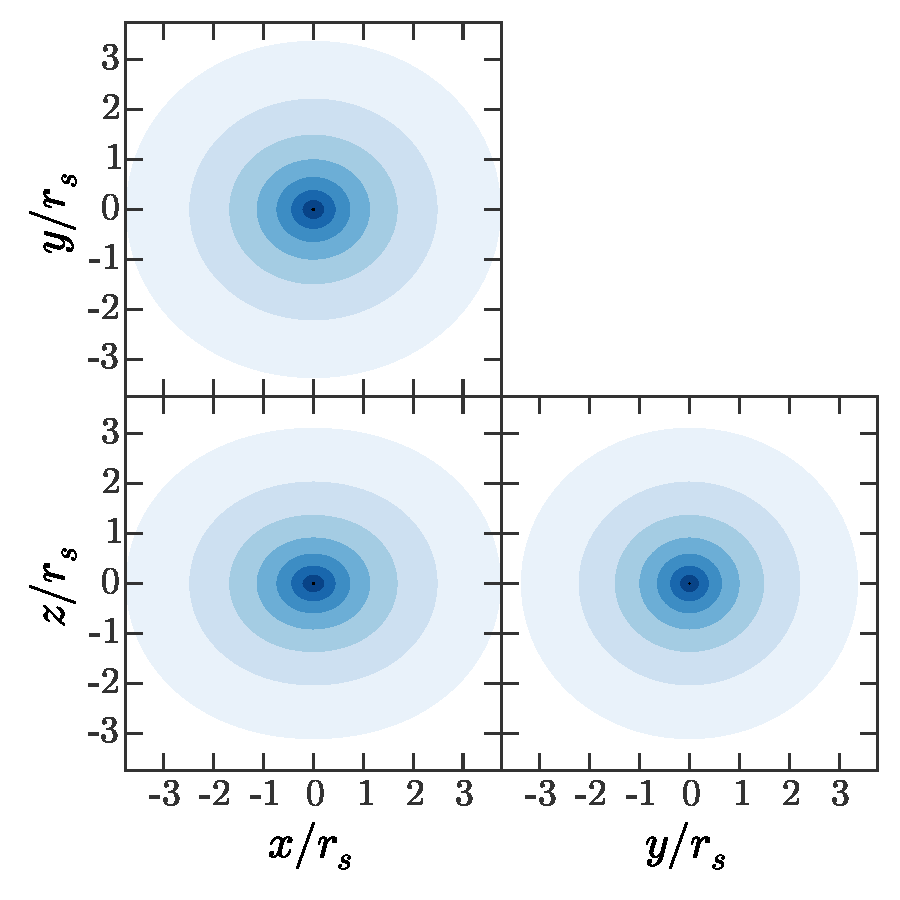
\includegraphics[width=0.75\textwidth]{figures/potential.pdf}
\caption{Rotation curve along $x$, $y$, and $z$ axes for the triaxial, NFW potential } \label{fig:orbit-tree}
\end{center}
\end{figure*}

[see discussion section for adding terms (disk, time evolution) to potential]

\subsection{Orbit integration}

[Use a blah blah integrator...]

\subsection{Lyapunov exponents}

The simplest and perhaps most well-known method for assessing chaotic motion is to analyze the Lyapunov spectrum or maximum Lyapunov exponent of an orbit. Defining the vector $\bs{w} = (q_1,...,q_N,p_1,...,p_N)$ for some set of canonical coordinates $(q_i,p_i)$, we can write Hamilton's equations as 
\begin{equation}
	\dot{\bs{w}} = \bs{\mathcal{J}} \frac{\partial H}{\partial \bs{w}} = f(\bs{w}) \label{eq:ham}
\end{equation}
where $\bs{\mathcal{J}}$ is the $2N \times 2N$ canonical Poisson tensor (also called the symplectic matrix) defined by
\begin{equation}
	\bs{\mathcal{J}} = \left( \begin{array}{c:c} 0 & \ident \\ \hdashline -\ident & 0 \end{array} \right)
\end{equation}
with $N$-dimensional identity matrices $\ident$. If we consider a nearby position separated from $\bs{w}$ by an infinitesimal deviation $\delta \bs{w}$, such that $\bs{w}' = \bs{w} + \delta \bs{w}$. We can expand to linear order in the deviation about the parent orbit and write the equations of motion for the deviation as follows
\begin{align}
	\dot{\bs{w}}' &= f(\bs{w}')\\
	\dot{\bs{w}} + \dot{\delta \bs{w}} &= f(\bs{w} +  \delta \bs{w})\\
	\dot{\bs{w}} + \dot{\delta \bs{w}} &\approx f(\bs{w}) + \jac_{\bs{w}}\cdot\delta \bs{w} + \mathcal{O}(\delta \bs{w}^2)\\
	\dot{\delta \bs{w}} &\approx \jac_{\bs{w}} \cdot  \delta \bs{w}\label{eq:deviate}
\end{align}
where $\jac$ is the Jacobian of Eq.~\ref{eq:ham}, evaluated at the parent orbit. For chaotic orbits, the maximum eigenvalue of the solution matrix to Eq.~\ref{eq:deviate} is positive real, leading to exponential divergence of nearby orbits. 

Computing the Lyapunov spectrum for a given orbit is often not necessary if one is only interested in characterizing the degree of chaos. Instead, it is often more efficient to compute the maximum Lyapunov exponent by estimating the finite-time maximum Lyapunov exponent (FTMLE), defined as 
\begin{equation}
	l_{\rm max}(t) = \frac{1}{t}\ln \frac{\|\delta \bs{w}(t)\|}{\|\delta \bs{w}_0\|}.\label{eq:lmax}
\end{equation}
The maximum Lyapunov exponent is the limit as $t\rightarrow \infty$ of the FTMLE
\begin{equation}
	\lambda_{\rm max} = \lim_{t\rightarrow\infty}l_{\rm max}(t). \label{eq:lyapmax}
\end{equation}
Numerically computing this quantity is not trivial because (1) obviously the limit to infinity is not possible and (2) the norm of the deviation vector $\|\delta \bs{w}(t)\|$ is expected to increase exponentially for chaotic orbits, leading to numerical problems. To circumvent these issues, it is sufficient to instead start a nearby orbit with some small initial deviation with norm $\delta_0$, integrate for a sufficiently small amount of time, $\tau$, then renormalize the deviation back to the initial norm (e.g., cite Bennetin et al. 1976, Tabor 1989). The following pseudocode outlines this procedure:\footnote{see Gary for Python implementation?}\\
\begin{algorithmic}[1]
\State {\bf define} orbital integration timestep, $h$, and number of steps, $K$
\State {\bf define} initial norm of deviation vector, $\delta_0$, to be sufficiently small
\State {\bf define} renormalization integration period, $\tau \ll hK$ 
\For{each timestep when integrating the main orbit, $\bs{w}(t)$}
\State step forward the orbit and deviation vector orbit by one timestep, $t_{i-1} \rightarrow t_i$
\If {a normalization timestep}
\State measure and store the length of the deviation vector, $\delta_i = \|\delta \bs{w}_i\|$
\State renormalize the length of the deviation vector, $\delta \bs{w}_i = \delta \bs{w}_i (\delta_0/\delta_i)$
\EndIf
\EndFor 
\end{algorithmic}
The FTMLE after a given number of timesteps, $N$, is then estimated as
\begin{equation}
	l_N = \frac{1}{N\tau}\sum_i^N \ln \, \delta_i
\end{equation}
and the MLE is
\begin{equation}
	\lambda_{\rm max} = \lim_{N\rightarrow \infty} l_N.
\end{equation}
[Some more practical issues with implementation] [Figure showing $l_N$ for regular, chaotic orbit?]

[Copy in text fomr ``behavior of MLE'']

[Computationally, expensive to compute Lyapunov exponent for sticky or mildly chaotic orbits]

\subsection{Numerical estimation of fundamental frequencies}

Bounded, regular orbits in triaxial potentials will have three \emph{fundamental frequencies}, $\bs{\Omega}$, that determine the periodic behavior of motion (Eq.~\ref{eq:aafreq}).

[Figure: reproduce some result?]

or
[Figure: for same orbits as in Lyapunov section, show frequency diffusion?]

\subsection{Particle balls}

Need a fast way to characterize morphology of local orbits after finite time

Can't run N-body for many tens of thousands of initial conditions

Explain simplistic approach

[Figure: Compare N-body simulation to balls of particles -- captures the essence]

Cite papers that use Lagrange-point stripping methods, Rewinder paper

Like only considering debris that comes off at a single pericentric passage

\section{Experiments}

\subsection{Frequency map}

We generate frequency maps at X energies for tube orbits started around the major and intermediate axes of the potential (figures)

Explain qualitative differences between the two -- e.g., Y-Z plane will have many more stochastic tubes because intermediate axis

\subsection{Morphology}

\subsubsection{Entropy evolution}

\subsubsection{Density evolution}

Compare mean density or some other metric for the balls, show that decreases faster for chaotic orbit -- chaotic mixing dominates over phase-mixing

Power law (Helmi and White)

\subsubsection{Adding a disk?}

\section{Discussion}\label{sec:discussion}

\subsection{Potential}

Time dependence

Radial dependence of axis ratios

Why not disk + bulge? What do we expect when we add? See later section for test of this...

\acknowledgements
APW is supported by a National Science Foundation Graduate Research Fellowship under Grant No.\ 11-44155. 
This research made use of Astropy, a community-developed core \texttt{Python} package for Astronomy \citep{astropy13}.
This work additionally relied on Columbia University's \emph{Hotfoot} and \emph{Yeti} compute clusters, and we acknowledge the Columbia HPC support staff for assistance. \\

\bibliographystyle{apj}
\bibliography{refs}

\end{document}
